\documentclass[11pt,a4paper]{article}

\usepackage[margin=2.4cm]{geometry}
\usepackage[T1]{fontenc}
\usepackage[utf8]{inputenc}
\usepackage{lmodern}
\usepackage{microtype}
\usepackage{graphicx}
\usepackage{booktabs}
\usepackage{tabularx}
\usepackage{array}
\usepackage{float}
\usepackage{xcolor}
\usepackage{hyperref}
\usepackage{caption}
\usepackage{subcaption}
\usepackage{enumitem}
\usepackage{siunitx}
\usepackage{amsmath}

\hypersetup{
  colorlinks=true,
  linkcolor=blue!50!black,
  citecolor=blue!50!black,
  urlcolor=blue!50!black
}

\graphicspath{{figures/}}
\setlist[itemize]{leftmargin=1.4em}
\setlist[enumerate]{leftmargin=1.6em}
\captionsetup{font=small, labelfont=bf}
\sisetup{round-mode=places, round-precision=2}

\newcolumntype{Y}{>{\raggedright\arraybackslash}X}
\newcommand{\code}[1]{\texttt{#1}}

\title{\textbf{Robust Mesh Quality Enhancement and Adaptive Remeshing}\\
\large CENG589 Digital Geometry Processing Term Project}
\author{Esad Mazi}
\date{\today}

\begin{document}
\maketitle

\begin{abstract}
Triangle meshes produced by CAD tessellators or other automatic conversion tools may contain very skinny or nearly degenerate triangles. These triangles are visually small, but they are harmful for geometry processing because they lead to unstable normals, poor numerical conditioning, and unreliable downstream operations. In this project, I implemented a mesh-quality pipeline inspired by Botsch and Kobbelt's robust degenerate-face removal procedure~\cite{botsch2001degenerate} and Dunyach et al.'s adaptive isotropic remeshing approach~\cite{dunyach2013adaptive}.

The implemented system reads OFF meshes, measures triangle quality, visualizes bad triangles, applies conservative remeshing operations, and finally removes remaining degenerate triangles using targeted local operations. The pipeline was tested on the provided joint model and two car models. On the joint model, the number of detected bad triangles was reduced from 258 to 0 while preserving closed topology. On the car models, the same cleanup idea removed almost all detected bad triangles without introducing non-manifold edges.
\end{abstract}

\section{Introduction}

The initial motivation of this project was practical rather than theoretical: the provided joint input mesh visibly contained many thin triangles, while the provided joint output mesh appeared to be a cleaned reference result. The main goal was therefore to build a reproducible pipeline that can explain, measure, and improve this difference.

The project follows three principles:
\begin{enumerate}
  \item Quality must be measured, not only inspected visually.
  \item Geometry processing operations must preserve topology whenever possible.
  \item Intermediate failures should be treated as observations, because they explain why more careful algorithms are necessary.
\end{enumerate}

This resulted in a pipeline that is intentionally simple but measurable. It does not try to be a complete industrial mesh repair system; instead, it focuses on a clear term-project scope: detect problematic triangles, improve them using local remeshing operations, compare the result against the provided reference output, and document the behavior on additional models.

\section{Background}

Botsch and Kobbelt classify degenerate triangles into two important categories: needles and caps~\cite{botsch2001degenerate}. Needles have very small angles and are usually long and thin. Caps have an angle close to \SI{180}{\degree}. The paper argues that these two cases should not be handled identically. In particular, needles can often be removed by collapsing short edges, while caps are more safely handled by splitting or slicing operations.

Dunyach et al. propose adaptive isotropic remeshing for interactive mesh deformation~\cite{dunyach2013adaptive}. Their key idea is to use a target edge length that changes over the surface: high-curvature regions should be sampled more densely, while flatter regions can be represented with larger triangles.

This project uses these ideas in a practical form:
\begin{itemize}
  \item triangle quality analysis and classification,
  \item conservative edge split and edge collapse operations,
  \item targeted cleanup for needles and caps,
  \item a curvature-based adaptive remeshing stage.
\end{itemize}

\section{Quality and Topology Metrics}

For each triangle, the implementation computes the minimum angle, maximum angle, shortest-edge / longest-edge aspect ratio, and near-zero area status. The thresholds used in the experiments are shown in Table~\ref{tab:labels}.

\begin{table}[H]
  \centering
  \caption{Bad triangle labels used in the experiments.}
  \label{tab:labels}
  \begin{tabularx}{0.92\linewidth}{lY}
    \toprule
    Label & Criterion \\
    \midrule
    Needle-like & Minimum angle below \SI{5}{\degree} or aspect ratio below 0.05 \\
    Cap-like & Maximum angle above \SI{175}{\degree} \\
    Near-zero area & Area below a scale-dependent epsilon \\
    \bottomrule
  \end{tabularx}
\end{table}

Topology is measured separately using boundary edge count, non-manifold edge count, and Euler characteristic. This separation became important during development. An early remeshing version improved some angle metrics but created holes and non-manifold edges. Therefore, the final pipeline reports both triangle quality and topology.

\section{Implementation}

The project is implemented in Python as a small command-line package named \code{meshfix}. The main modules are summarized in Table~\ref{tab:modules}.

\begin{table}[H]
  \centering
  \caption{Main implementation modules.}
  \label{tab:modules}
  \begin{tabularx}{0.95\linewidth}{lY}
    \toprule
    Module & Purpose \\
    \midrule
    \code{meshfix.io} & OFF mesh reading and writing \\
    \code{meshfix.quality} & Triangle quality metrics and bad triangle classification \\
    \code{meshfix.visualize} & Colored PLY export and Polyscope visualization \\
    \code{meshfix.topology} & Boundary and non-manifold edge analysis \\
    \code{meshfix.remesh} & Uniform and adaptive remeshing operations \\
    \code{meshfix.cleanup} & Targeted needle/cap cleanup \\
    \code{meshfix.curvature} & Curvature proxy and adaptive sizing field \\
    \bottomrule
  \end{tabularx}
\end{table}

Bad triangles are visualized with a simple color scheme: gray for acceptable triangles, red for needle-like triangles, orange for low aspect ratio triangles, purple for cap-like triangles, and black for near-zero area triangles.

\section{Method}

\subsection{Baseline Analysis}

The first step is to read the input OFF mesh and compute quality statistics without changing the geometry. This gives an objective baseline for comparison. For example, \code{joint\_input.off} contains 258 detected bad triangles, while the provided \code{joint\_output.off} contains none under the same thresholds.

\begin{figure}[H]
  \centering
  \begin{subfigure}{0.48\linewidth}
    \centering
    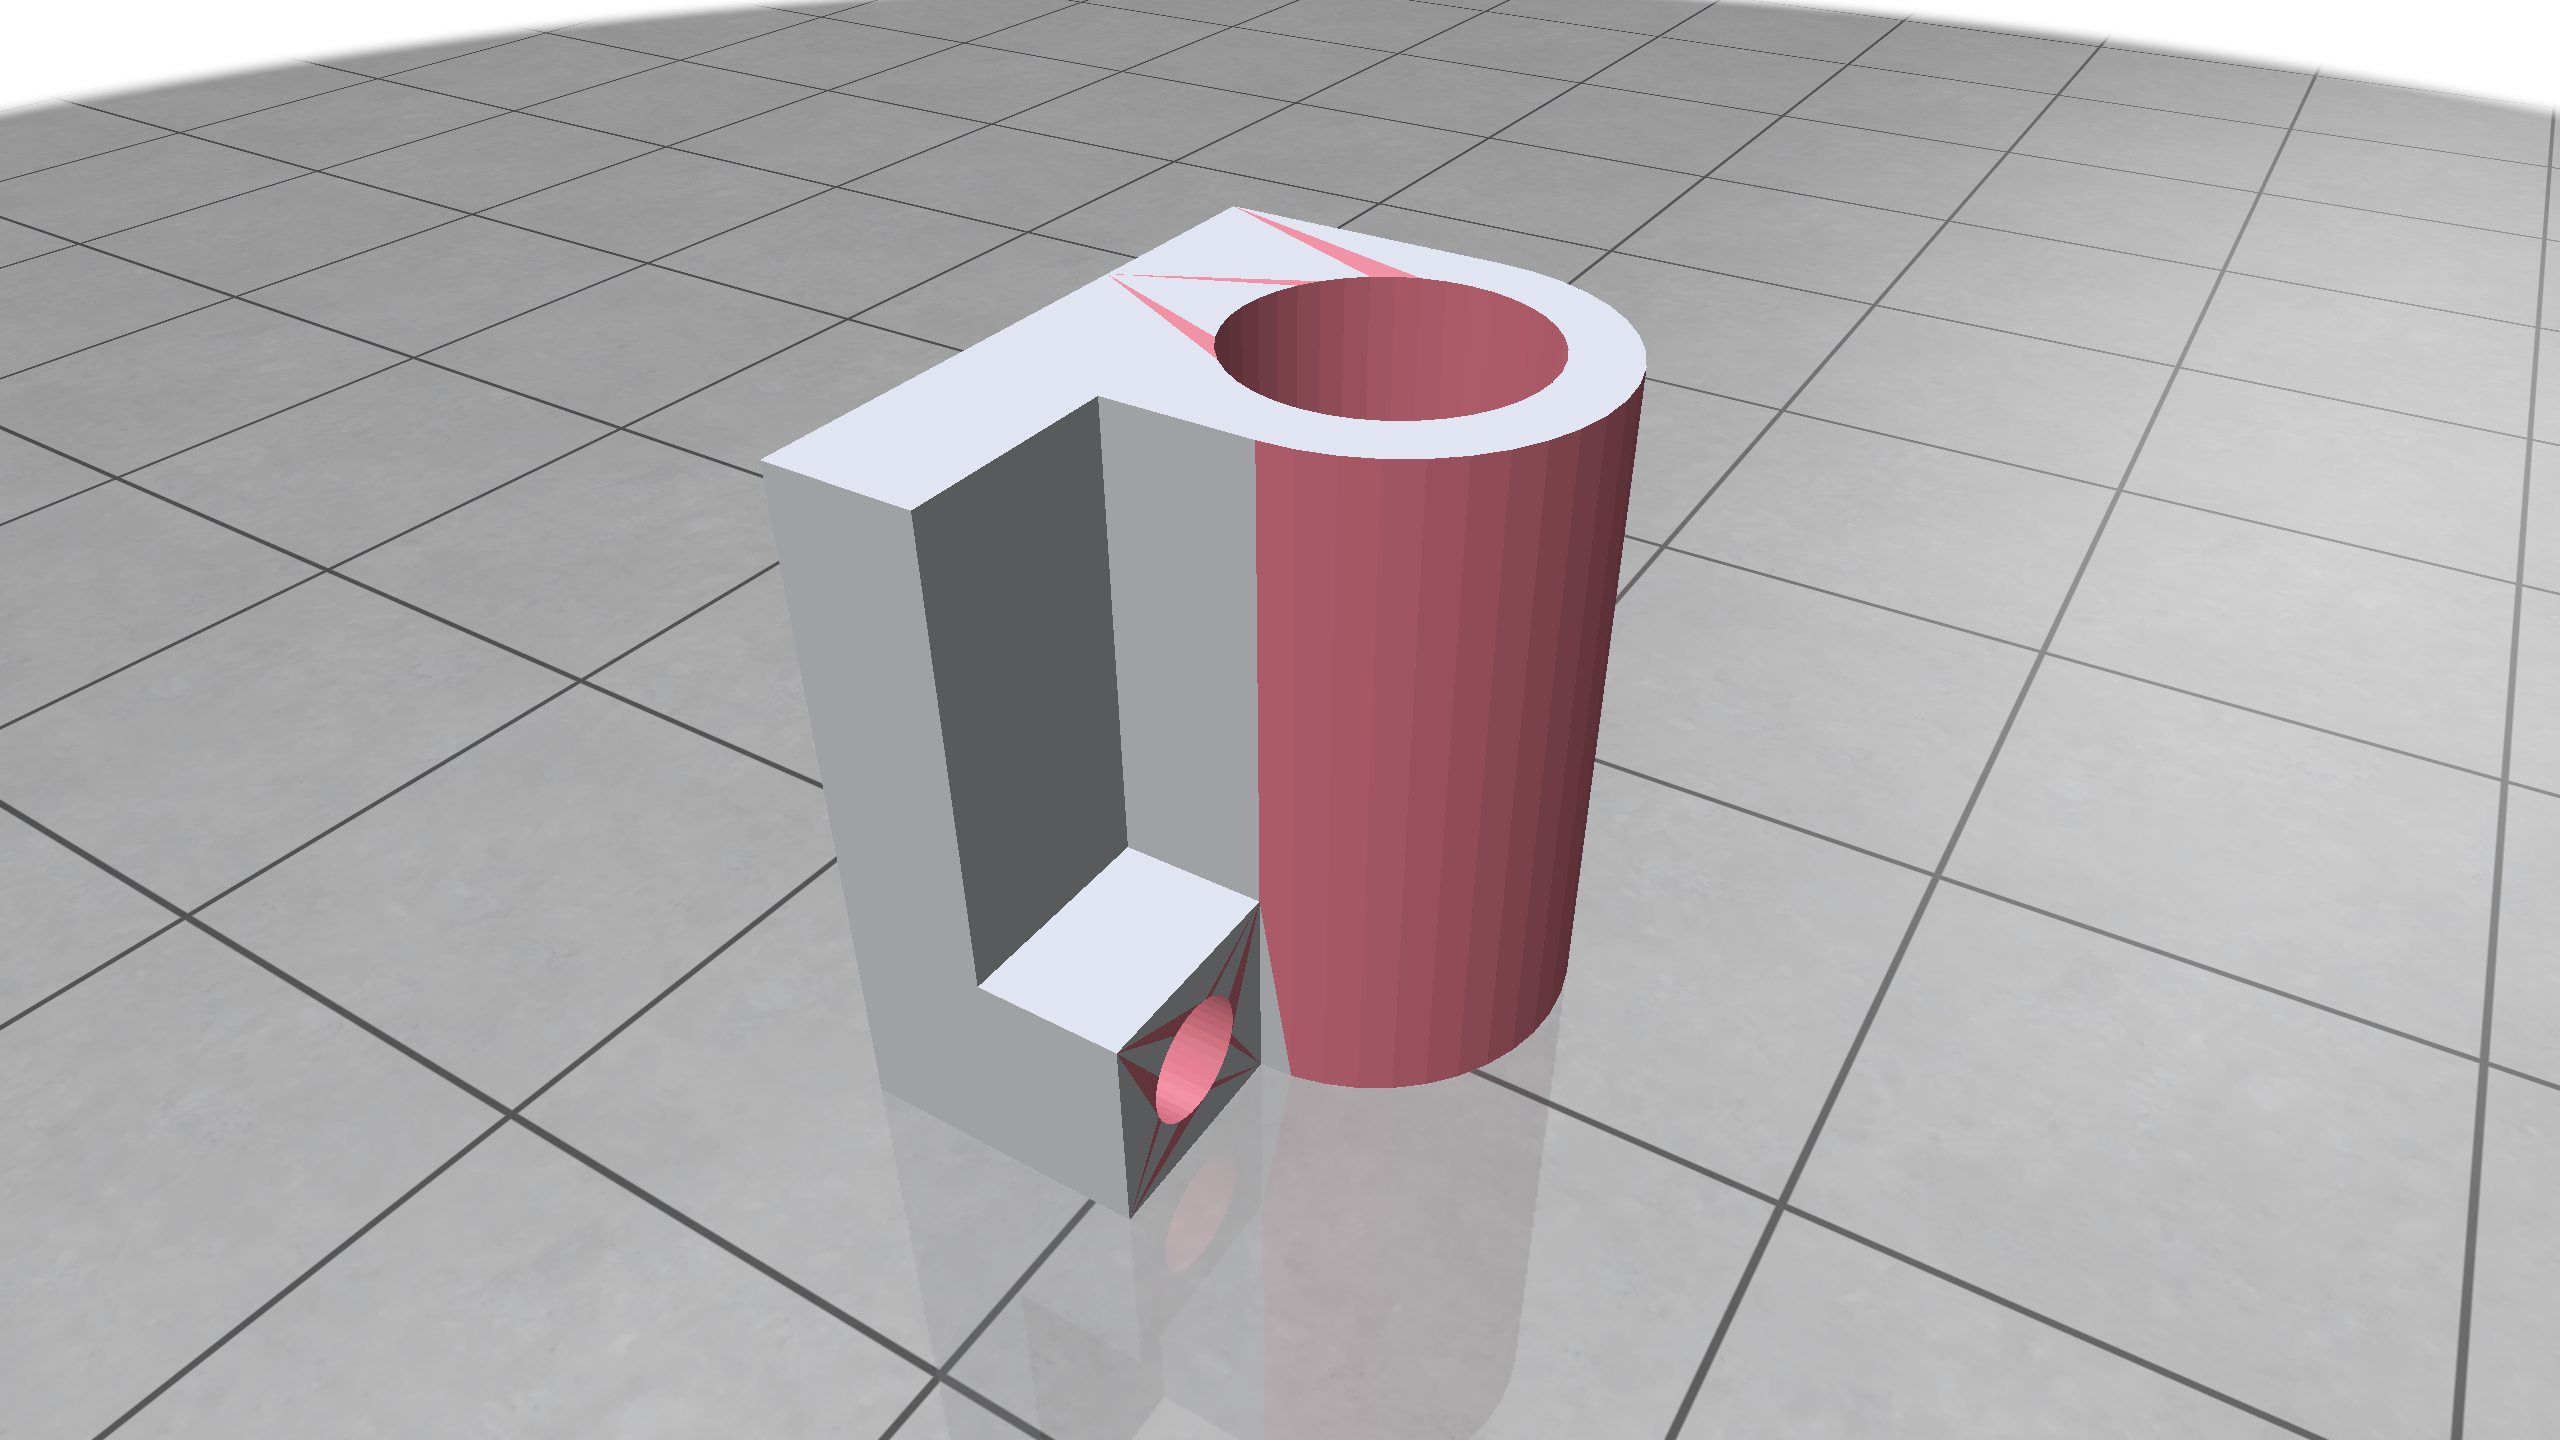
\includegraphics[width=\linewidth]{fig01_joint_input_quality.png}
    \caption{\code{joint\_input.off}}
  \end{subfigure}
  \hfill
  \begin{subfigure}{0.48\linewidth}
    \centering
    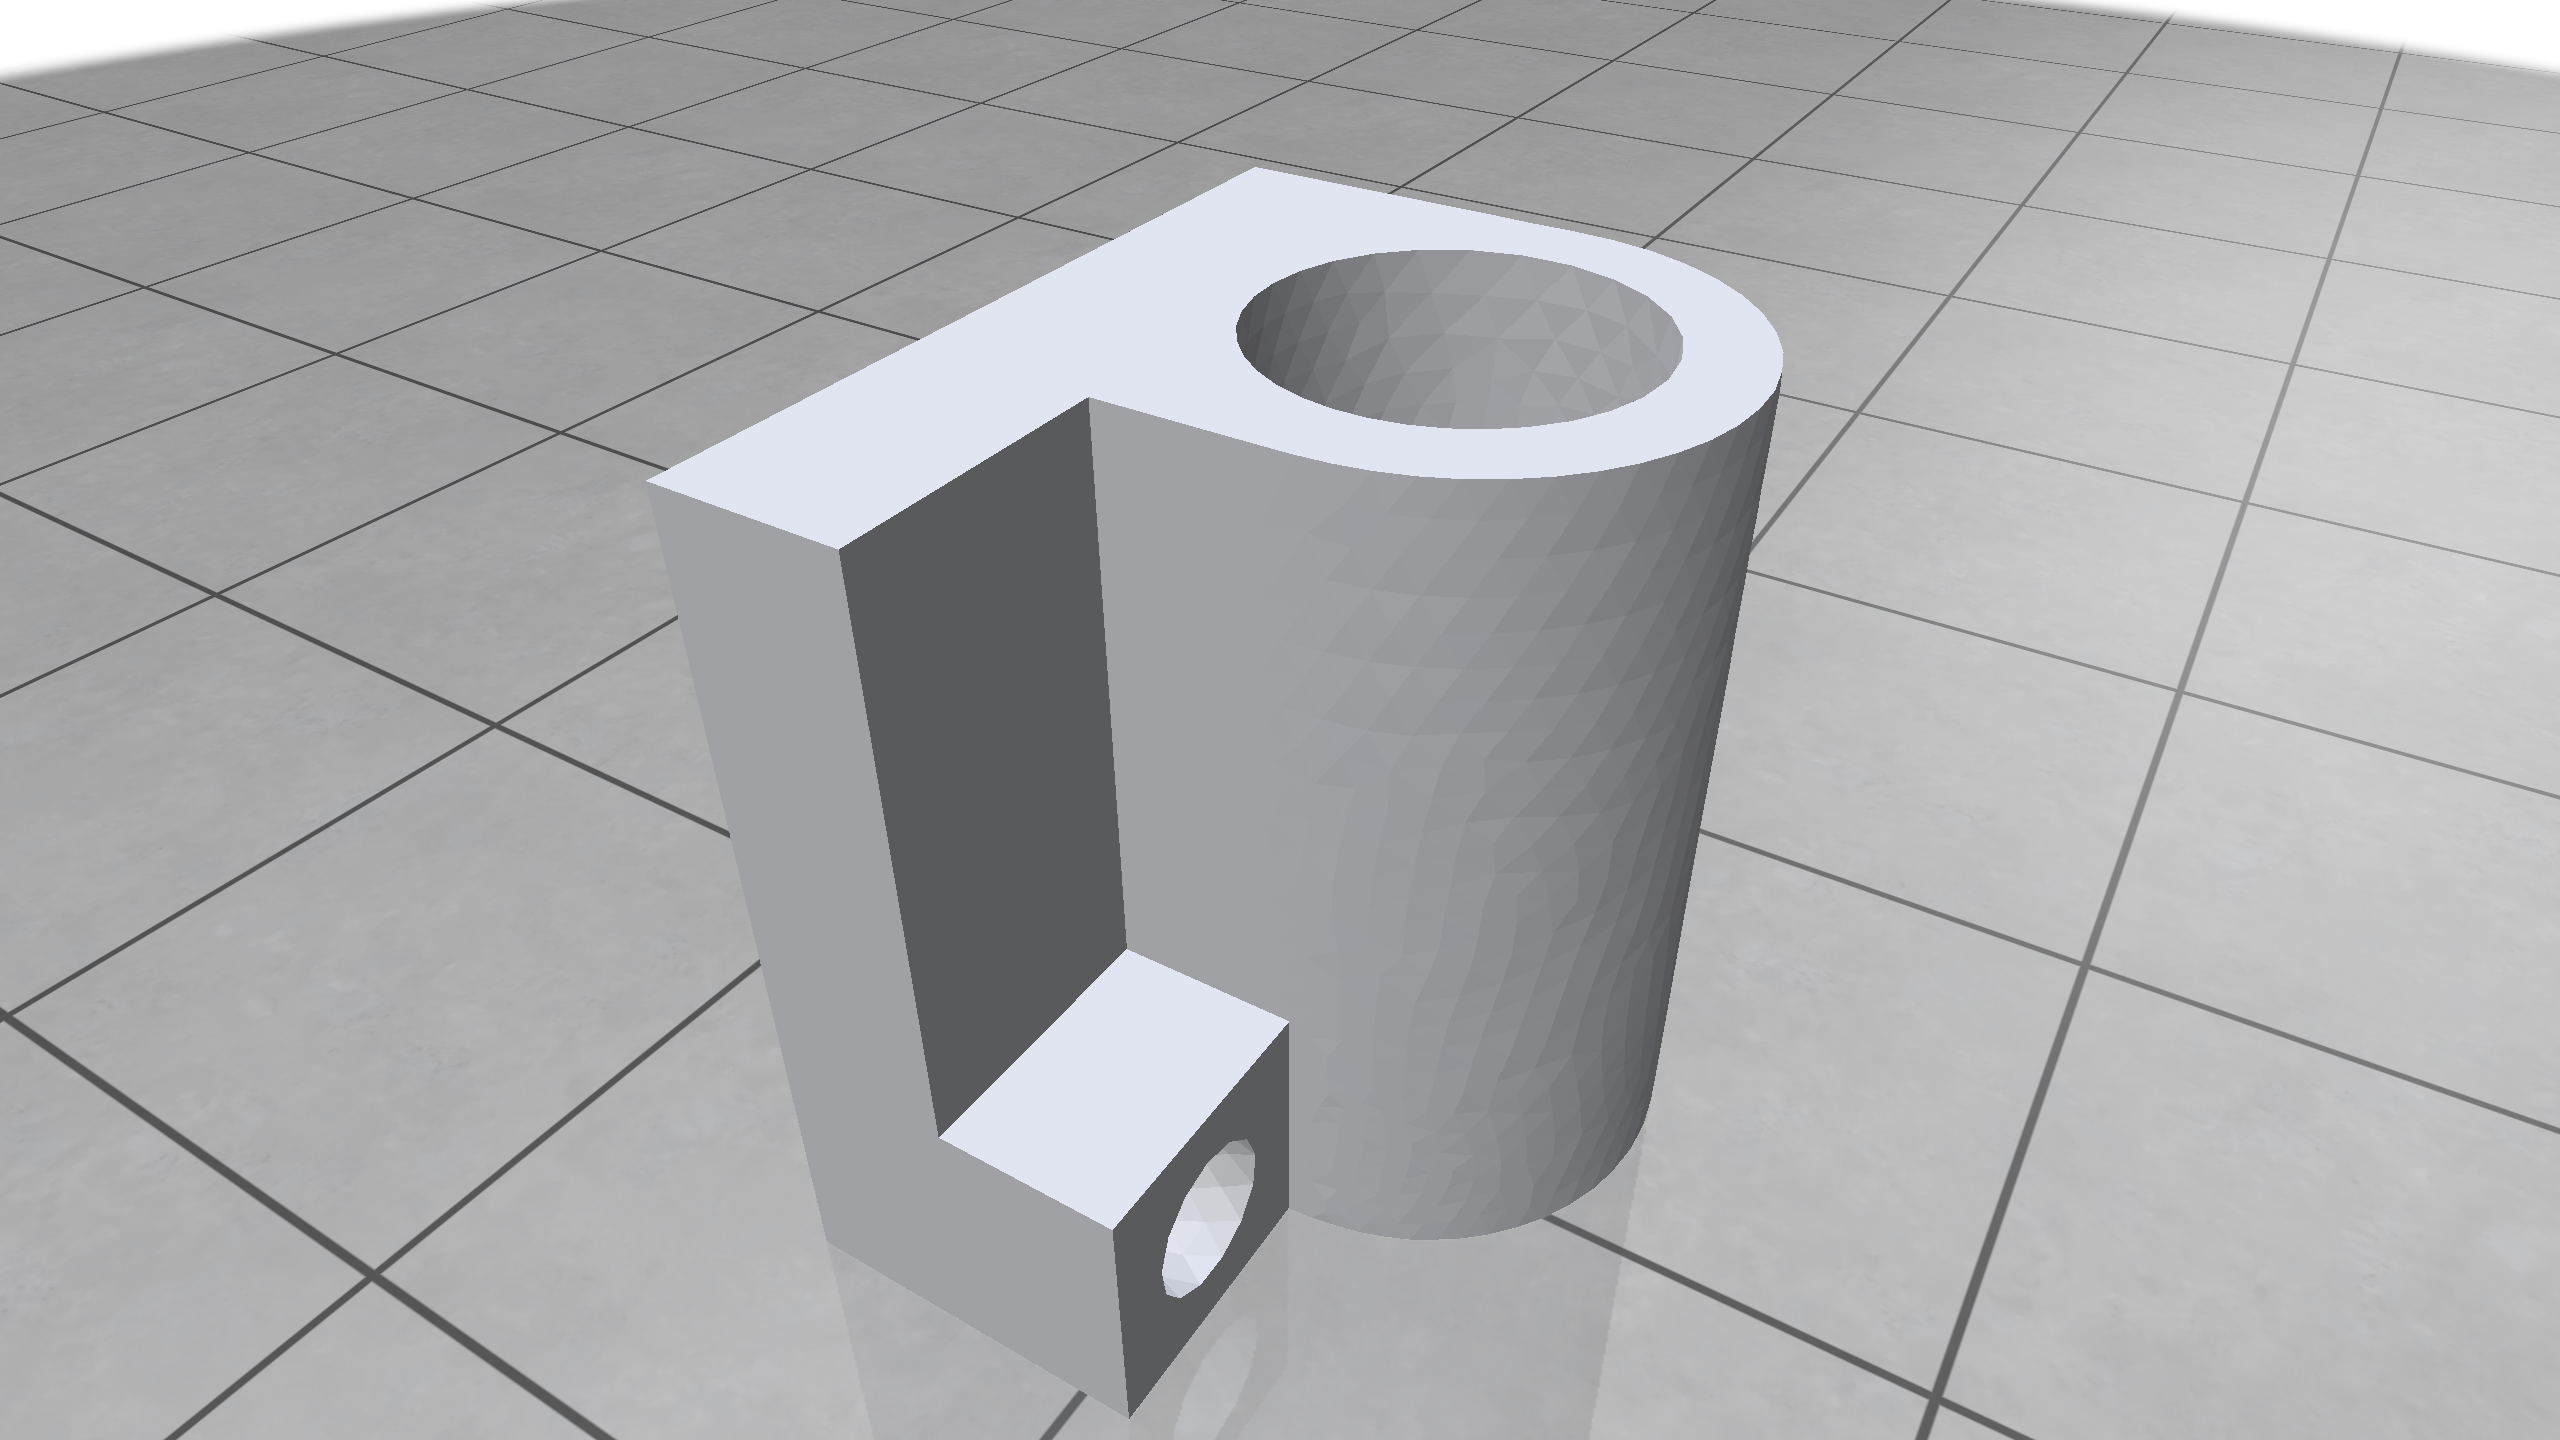
\includegraphics[width=\linewidth]{fig02_joint_instructor_output_quality.png}
    \caption{\code{joint\_output.off}}
  \end{subfigure}
  \caption{Baseline quality visualization of the provided joint meshes. Red triangles indicate needle-like degenerate triangles, while gray triangles pass the quality tests.}
  \label{fig:joint-baseline}
\end{figure}

\subsection{Conservative Uniform Remeshing}

The first remeshing stage attempts to regularize edge lengths using local operations: split edges that are too long, collapse edges that are too short, and reject operations that would create invalid topology.

The initial implementation was intentionally tested visually and numerically. It revealed a common remeshing problem: splitting one triangle without consistently splitting its neighbor can create cracks or T-junction-like artifacts. This was fixed by globally consistent edge splitting, where all triangles sharing a split edge use the same midpoint.

Another issue appeared with aggressive smoothing and edge flips. They improved some angle statistics but caused visible deformation and small topology defects. For this reason, the final uniform remeshing baseline uses conservative split and collapse operations, while flip and smoothing are kept as optional experimental flags.

\begin{figure}[H]
  \centering
  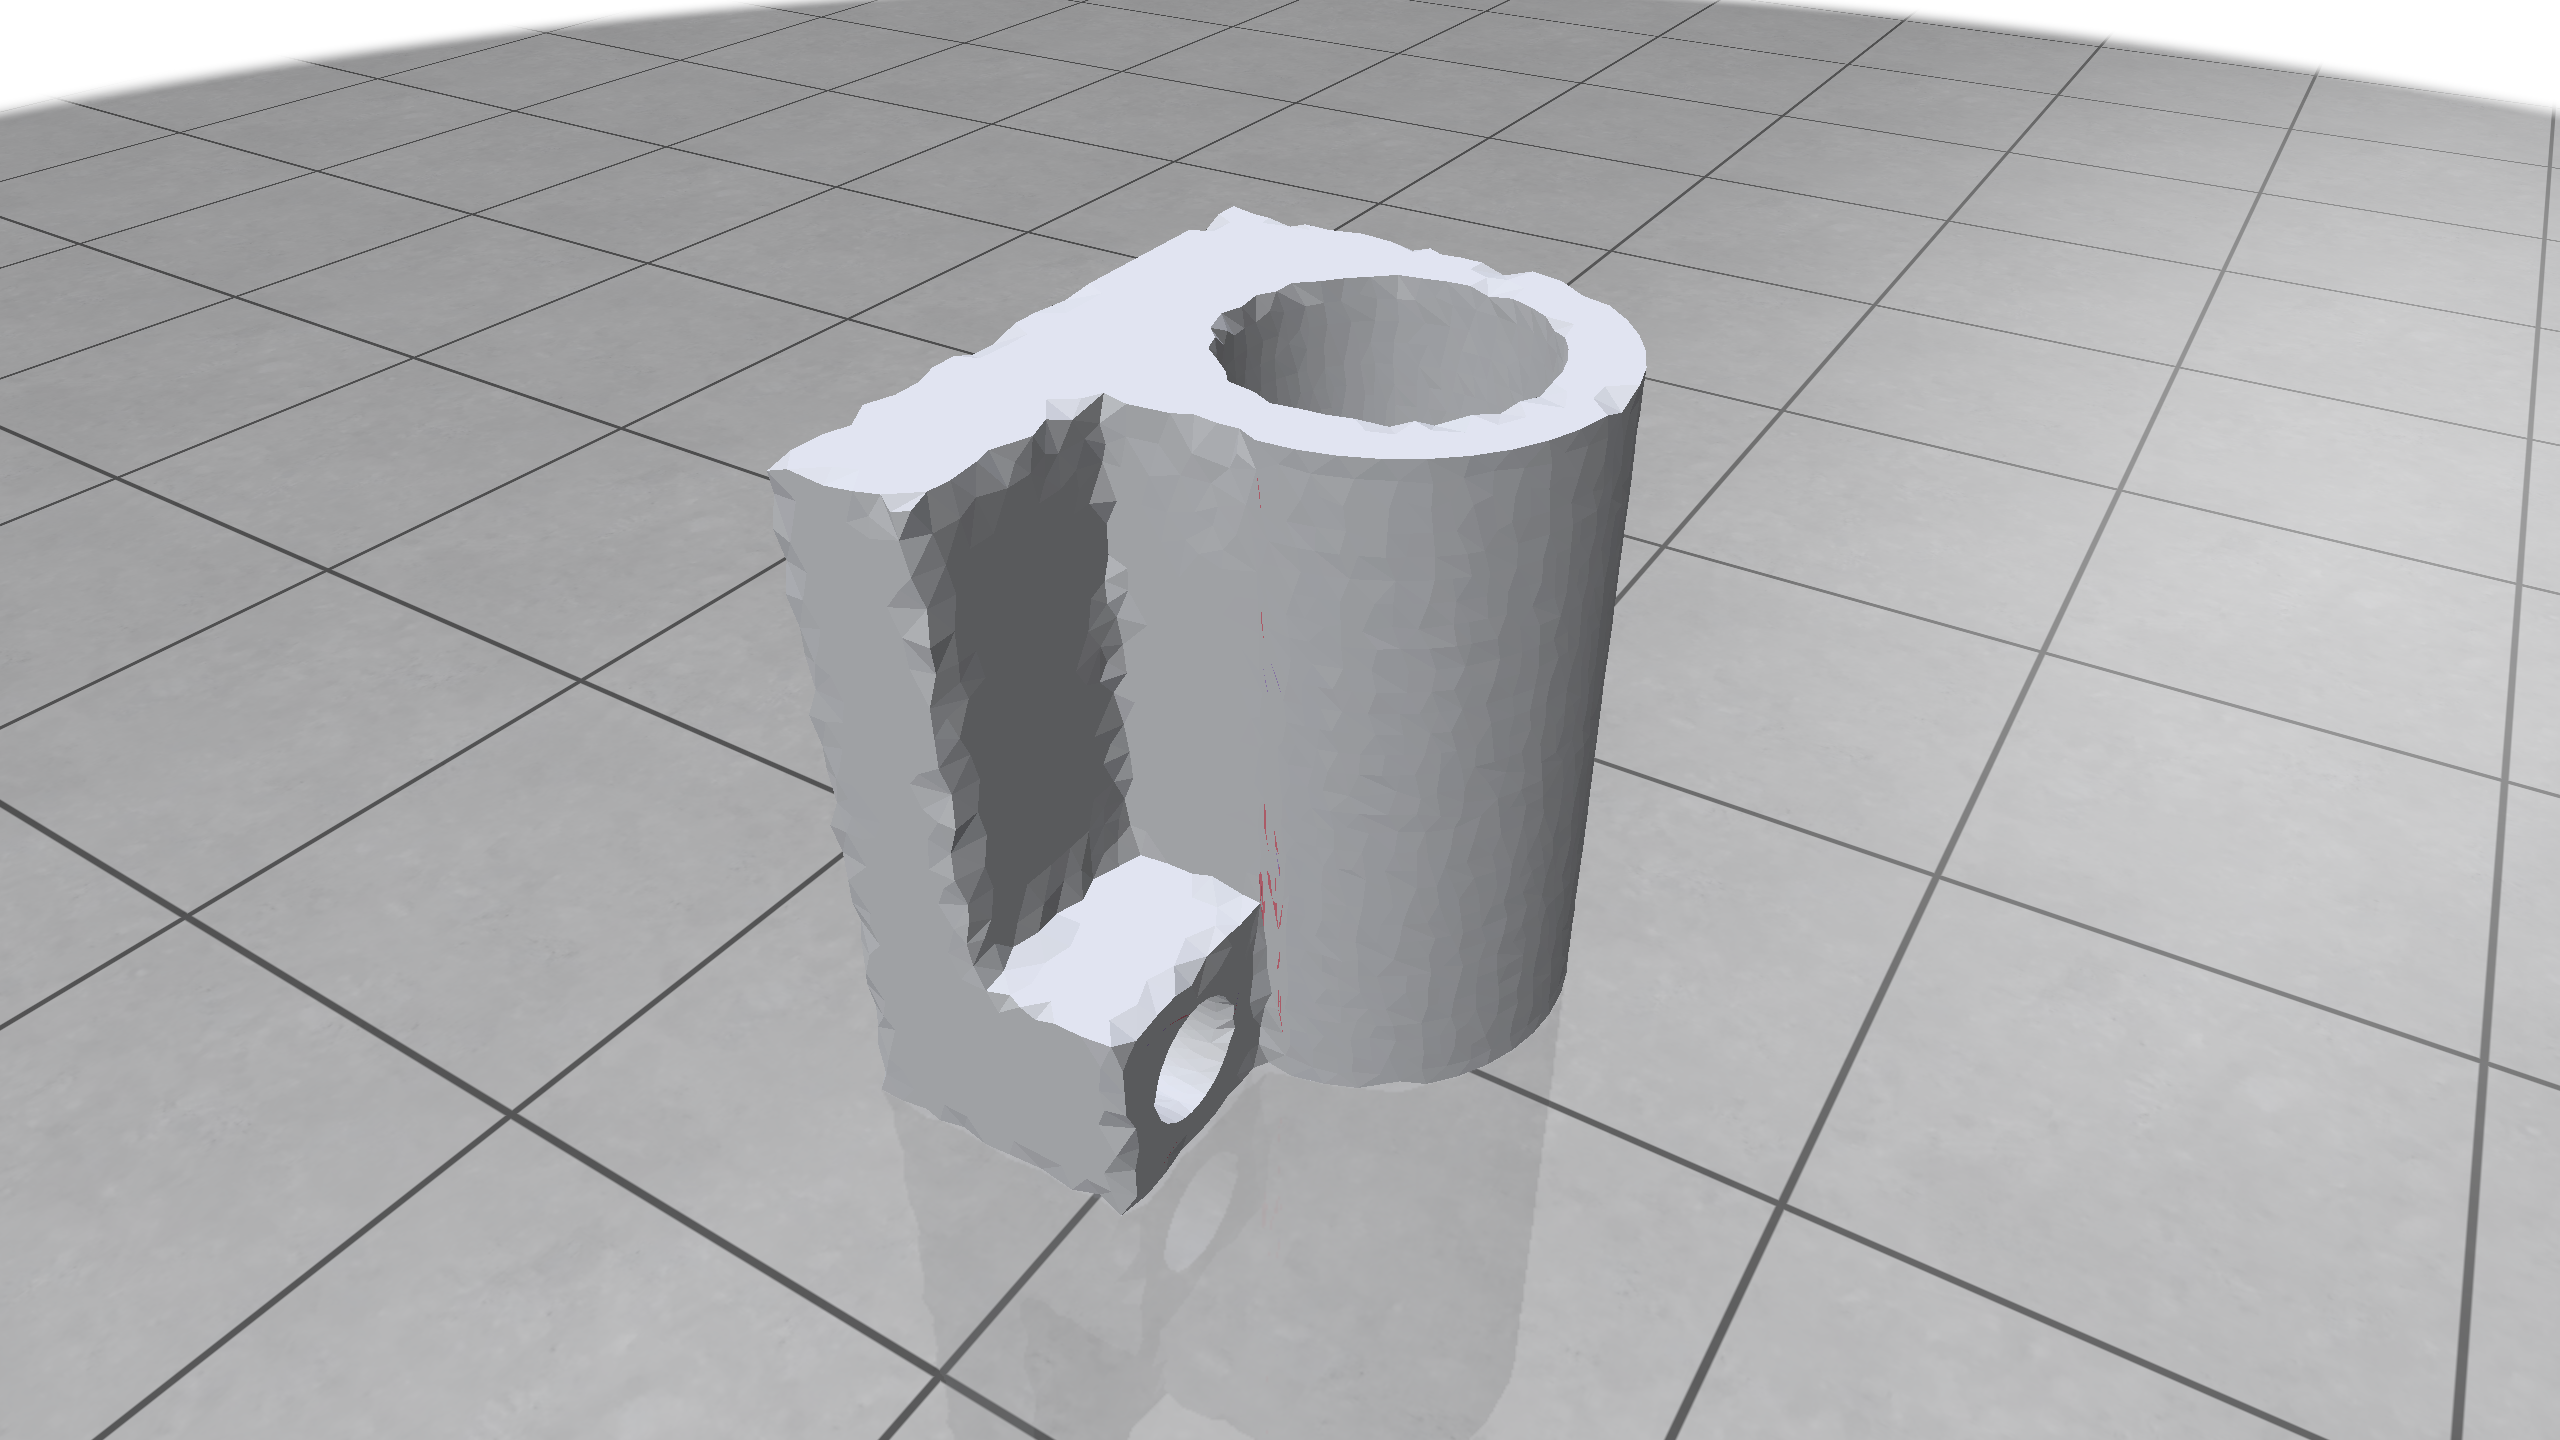
\includegraphics[width=0.72\linewidth]{fig03_joint_uniform_safe_quality.png}
  \caption{Conservative uniform remeshing result. The number of bad triangles is greatly reduced, but some red and purple triangles remain.}
  \label{fig:uniform-safe}
\end{figure}

\subsection{Targeted Degenerate Cleanup}

Uniform remeshing alone does not remove all degenerate triangles. The next stage uses the distinction between needles and caps:
\begin{itemize}
  \item for needle-like triangles, collapse the shortest edge;
  \item for cap-like triangles, split the longest edge.
\end{itemize}

Each candidate operation is checked before it is accepted. Operations that would introduce non-manifold edges or boundary changes on closed meshes are rejected. This targeted cleanup stage reduced the remaining bad triangles on the joint model from 43 to 0.

\subsection{Adaptive Remeshing}

The adaptive stage follows the idea of Dunyach et al. by replacing a single global target edge length with a local sizing field. I implemented a simple curvature proxy based on vertex normal variation over one-ring edges. The resulting rule is:
\begin{itemize}
  \item high normal variation: smaller target edge length;
  \item low normal variation: larger target edge length.
\end{itemize}

On the joint model, adaptive remeshing improved the average minimum angle and reduced the number of triangles compared to the uniform-cleanup result. A final targeted cleanup pass was then applied to remove the few bad triangles created by adaptive operations.

\begin{figure}[H]
  \centering
  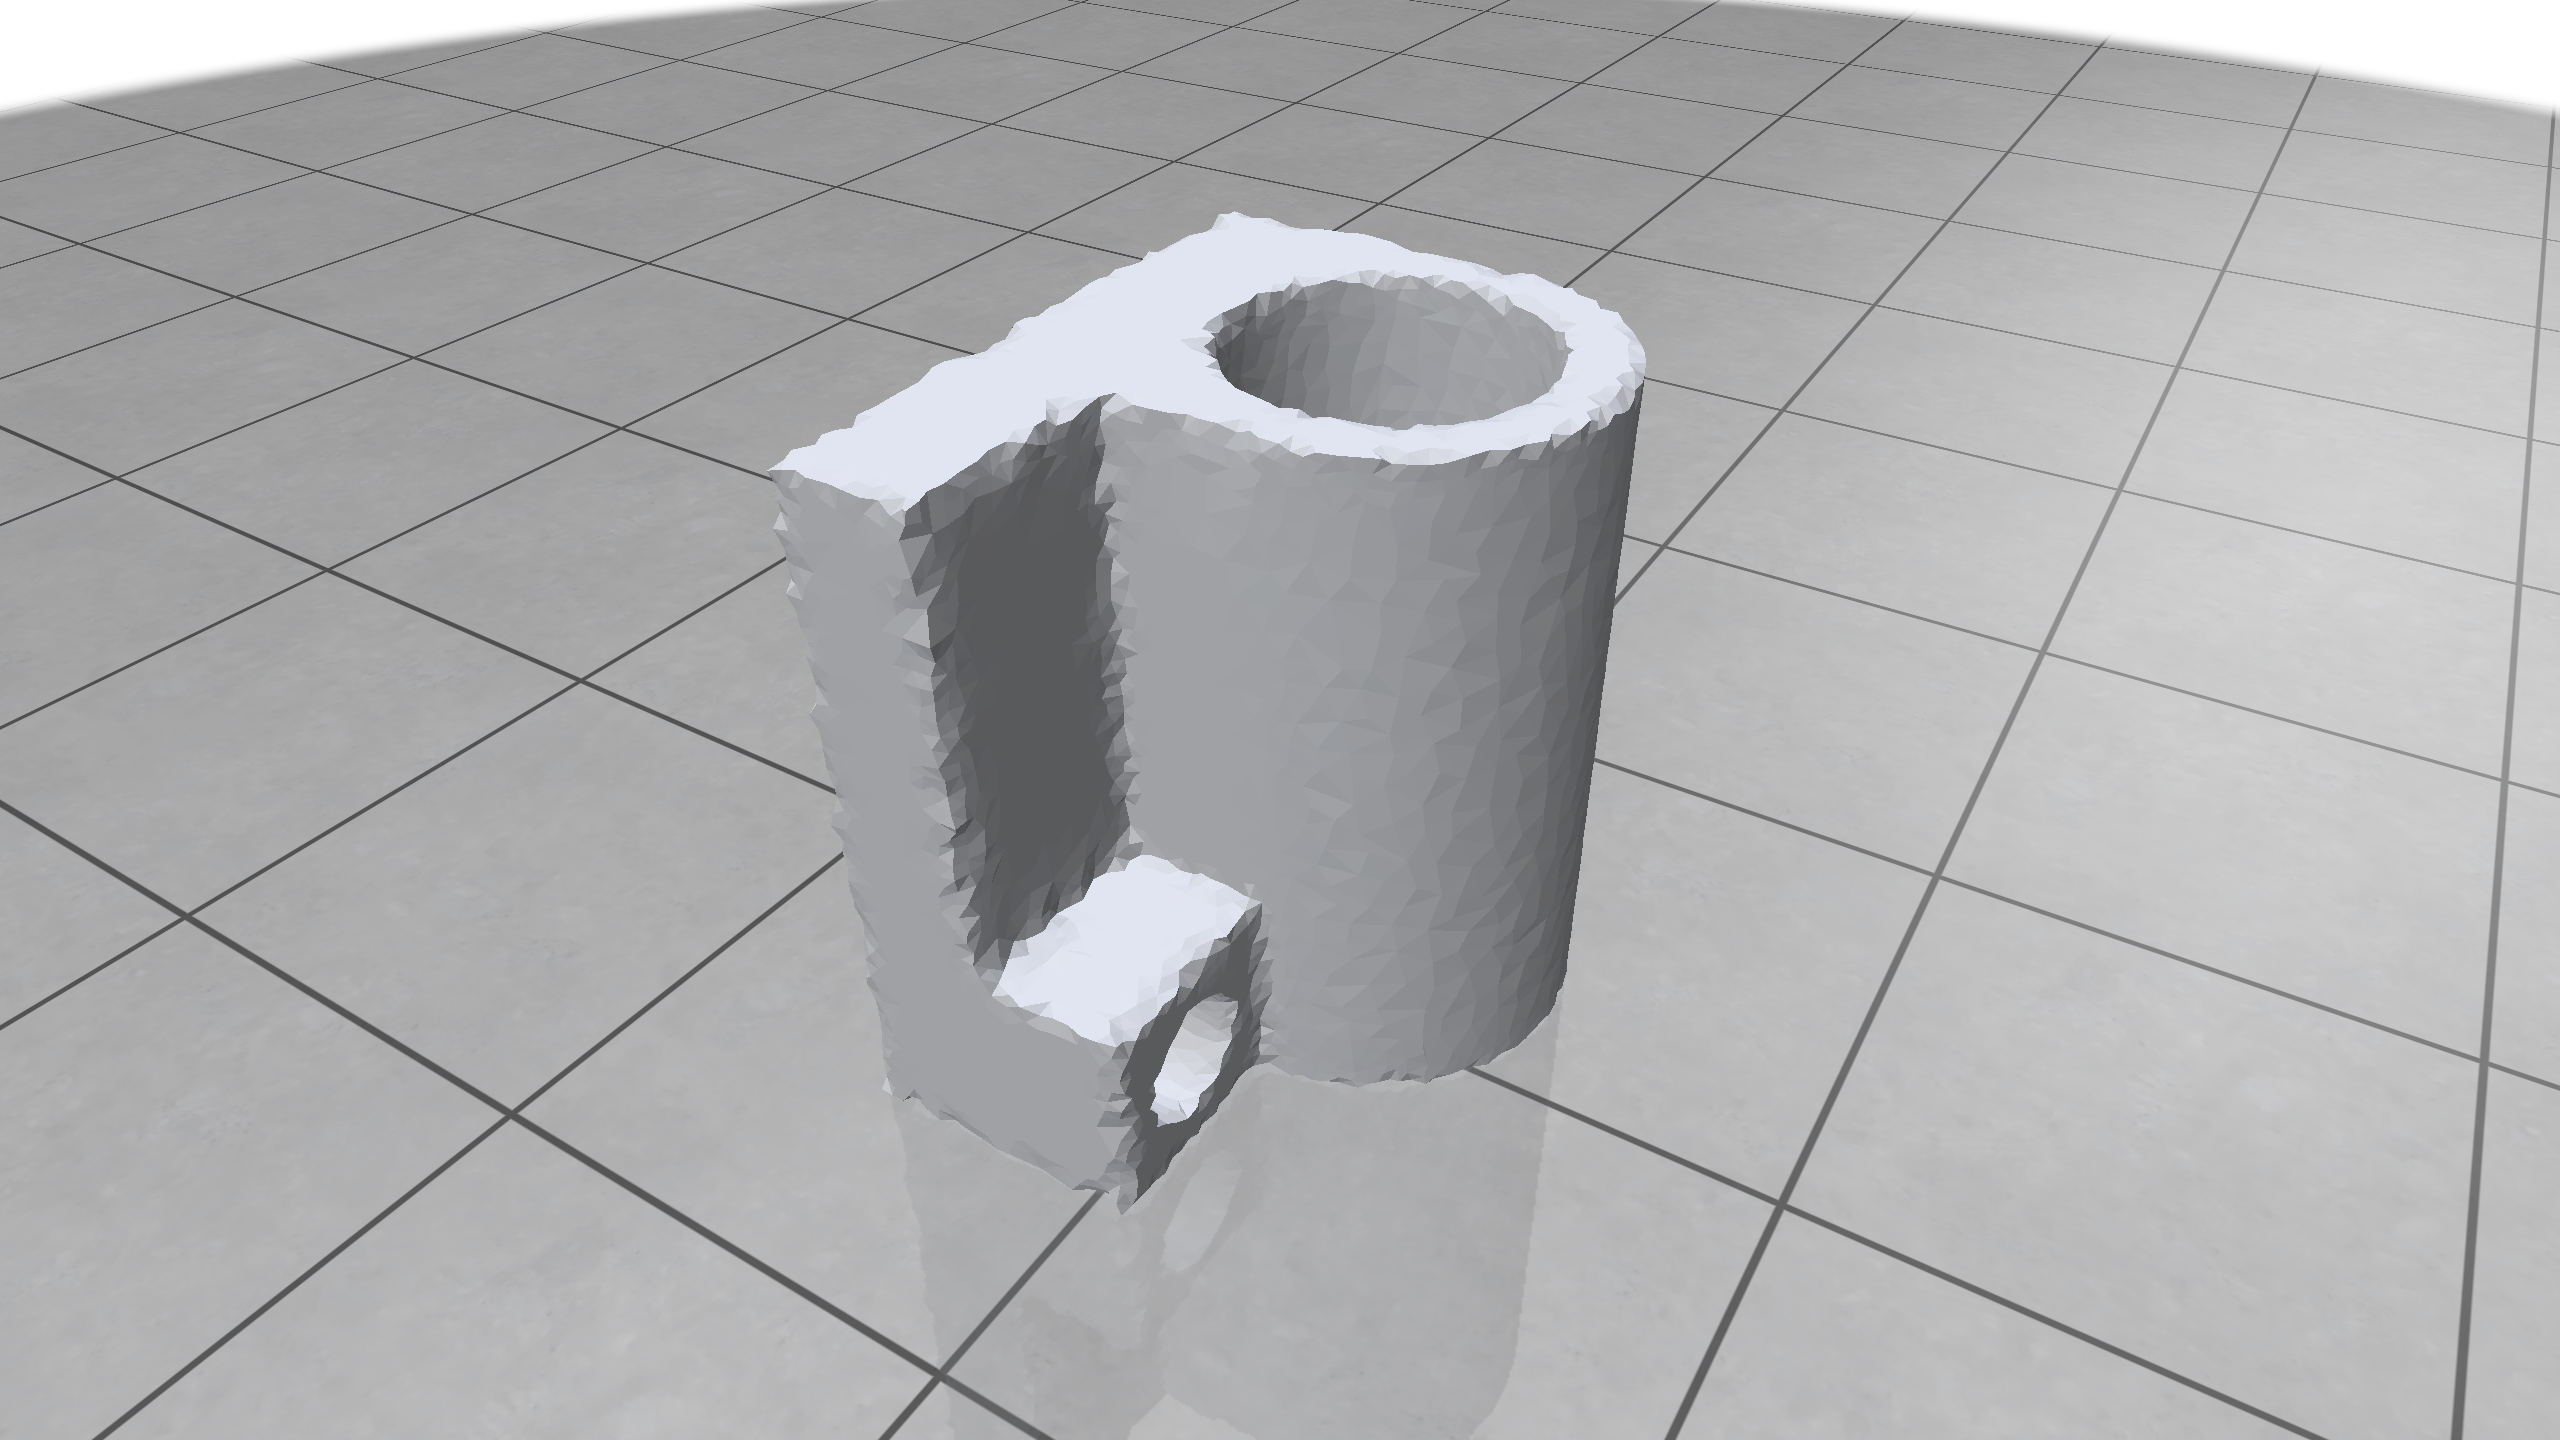
\includegraphics[width=0.72\linewidth]{fig04_joint_adaptive_final_quality.png}
  \caption{Final result of the implemented pipeline on the joint model. All detected bad triangles are removed and the topology remains clean.}
  \label{fig:joint-final}
\end{figure}

\section{Results}

\subsection{Joint Model}

\begin{table}[H]
  \centering
  \caption{Joint model results. Angles are in degrees.}
  \label{tab:joint-results}
  \resizebox{\linewidth}{!}{%
  \begin{tabular}{lrrrrrrr}
    \toprule
    Mesh & V & F & Min angle & Avg min angle & Bad triangles & Boundary & Non-manifold \\
    \midrule
    \code{joint\_input.off} & 221 & 446 & 0.48 & 9.35 & 258 & 0 & 0 \\
    \code{joint\_uniform\_safe.off} & 6537 & 13078 & 0.06 & 35.19 & 43 & 0 & 0 \\
    \code{joint\_adaptive\_final.off} & 6061 & 12126 & 5.65 & 42.13 & 0 & 0 & 0 \\
    \code{joint\_output.off} & 3400 & 6804 & 36.00 & 53.00 & 0 & 0 & 0 \\
    \bottomrule
  \end{tabular}}
\end{table}

The final adaptive result reaches the same bad-triangle count as the instructor reference output: zero. It does not exactly reproduce the reference mesh, and it uses more triangles, but it demonstrates the intended cleanup behavior with a fully implemented and reproducible pipeline.

\subsection{Car Models}

The car models are already much denser than the joint model. For these meshes, targeted cleanup was more practical than full adaptive remeshing. Direct adaptive remeshing on \code{car4} over-refined the mesh and became computationally expensive, so it was not used as the final car-model pipeline.

\begin{table}[H]
  \centering
  \caption{Car model results. Angles are in degrees.}
  \label{tab:car-results}
  \resizebox{\linewidth}{!}{%
  \begin{tabular}{lrrrrrrr}
    \toprule
    Mesh & V & F & Min angle & Avg min angle & Bad triangles & Boundary & Non-manifold \\
    \midrule
    \code{car1.off} & 48798 & 97536 & 0.73 & 27.04 & 1400 & 64 & 0 \\
    \code{car1\_cleanup.off} & 48349 & 96638 & 4.64 & 27.28 & 4 & 64 & 0 \\
    \code{car4.off} & 14317 & 28630 & 0.59 & 18.76 & 4787 & 0 & 0 \\
    \code{car4\_cleanup.off} & 12308 & 24612 & 0.95 & 21.68 & 5 & 0 & 0 \\
    \bottomrule
  \end{tabular}}
\end{table}

For \code{car1}, the original mesh already has 64 boundary edges. The cleanup stage preserves this count and does not introduce non-manifold edges. For \code{car4}, the mesh starts closed and remains closed.

\begin{figure}[H]
  \centering
  \begin{subfigure}{0.48\linewidth}
    \centering
    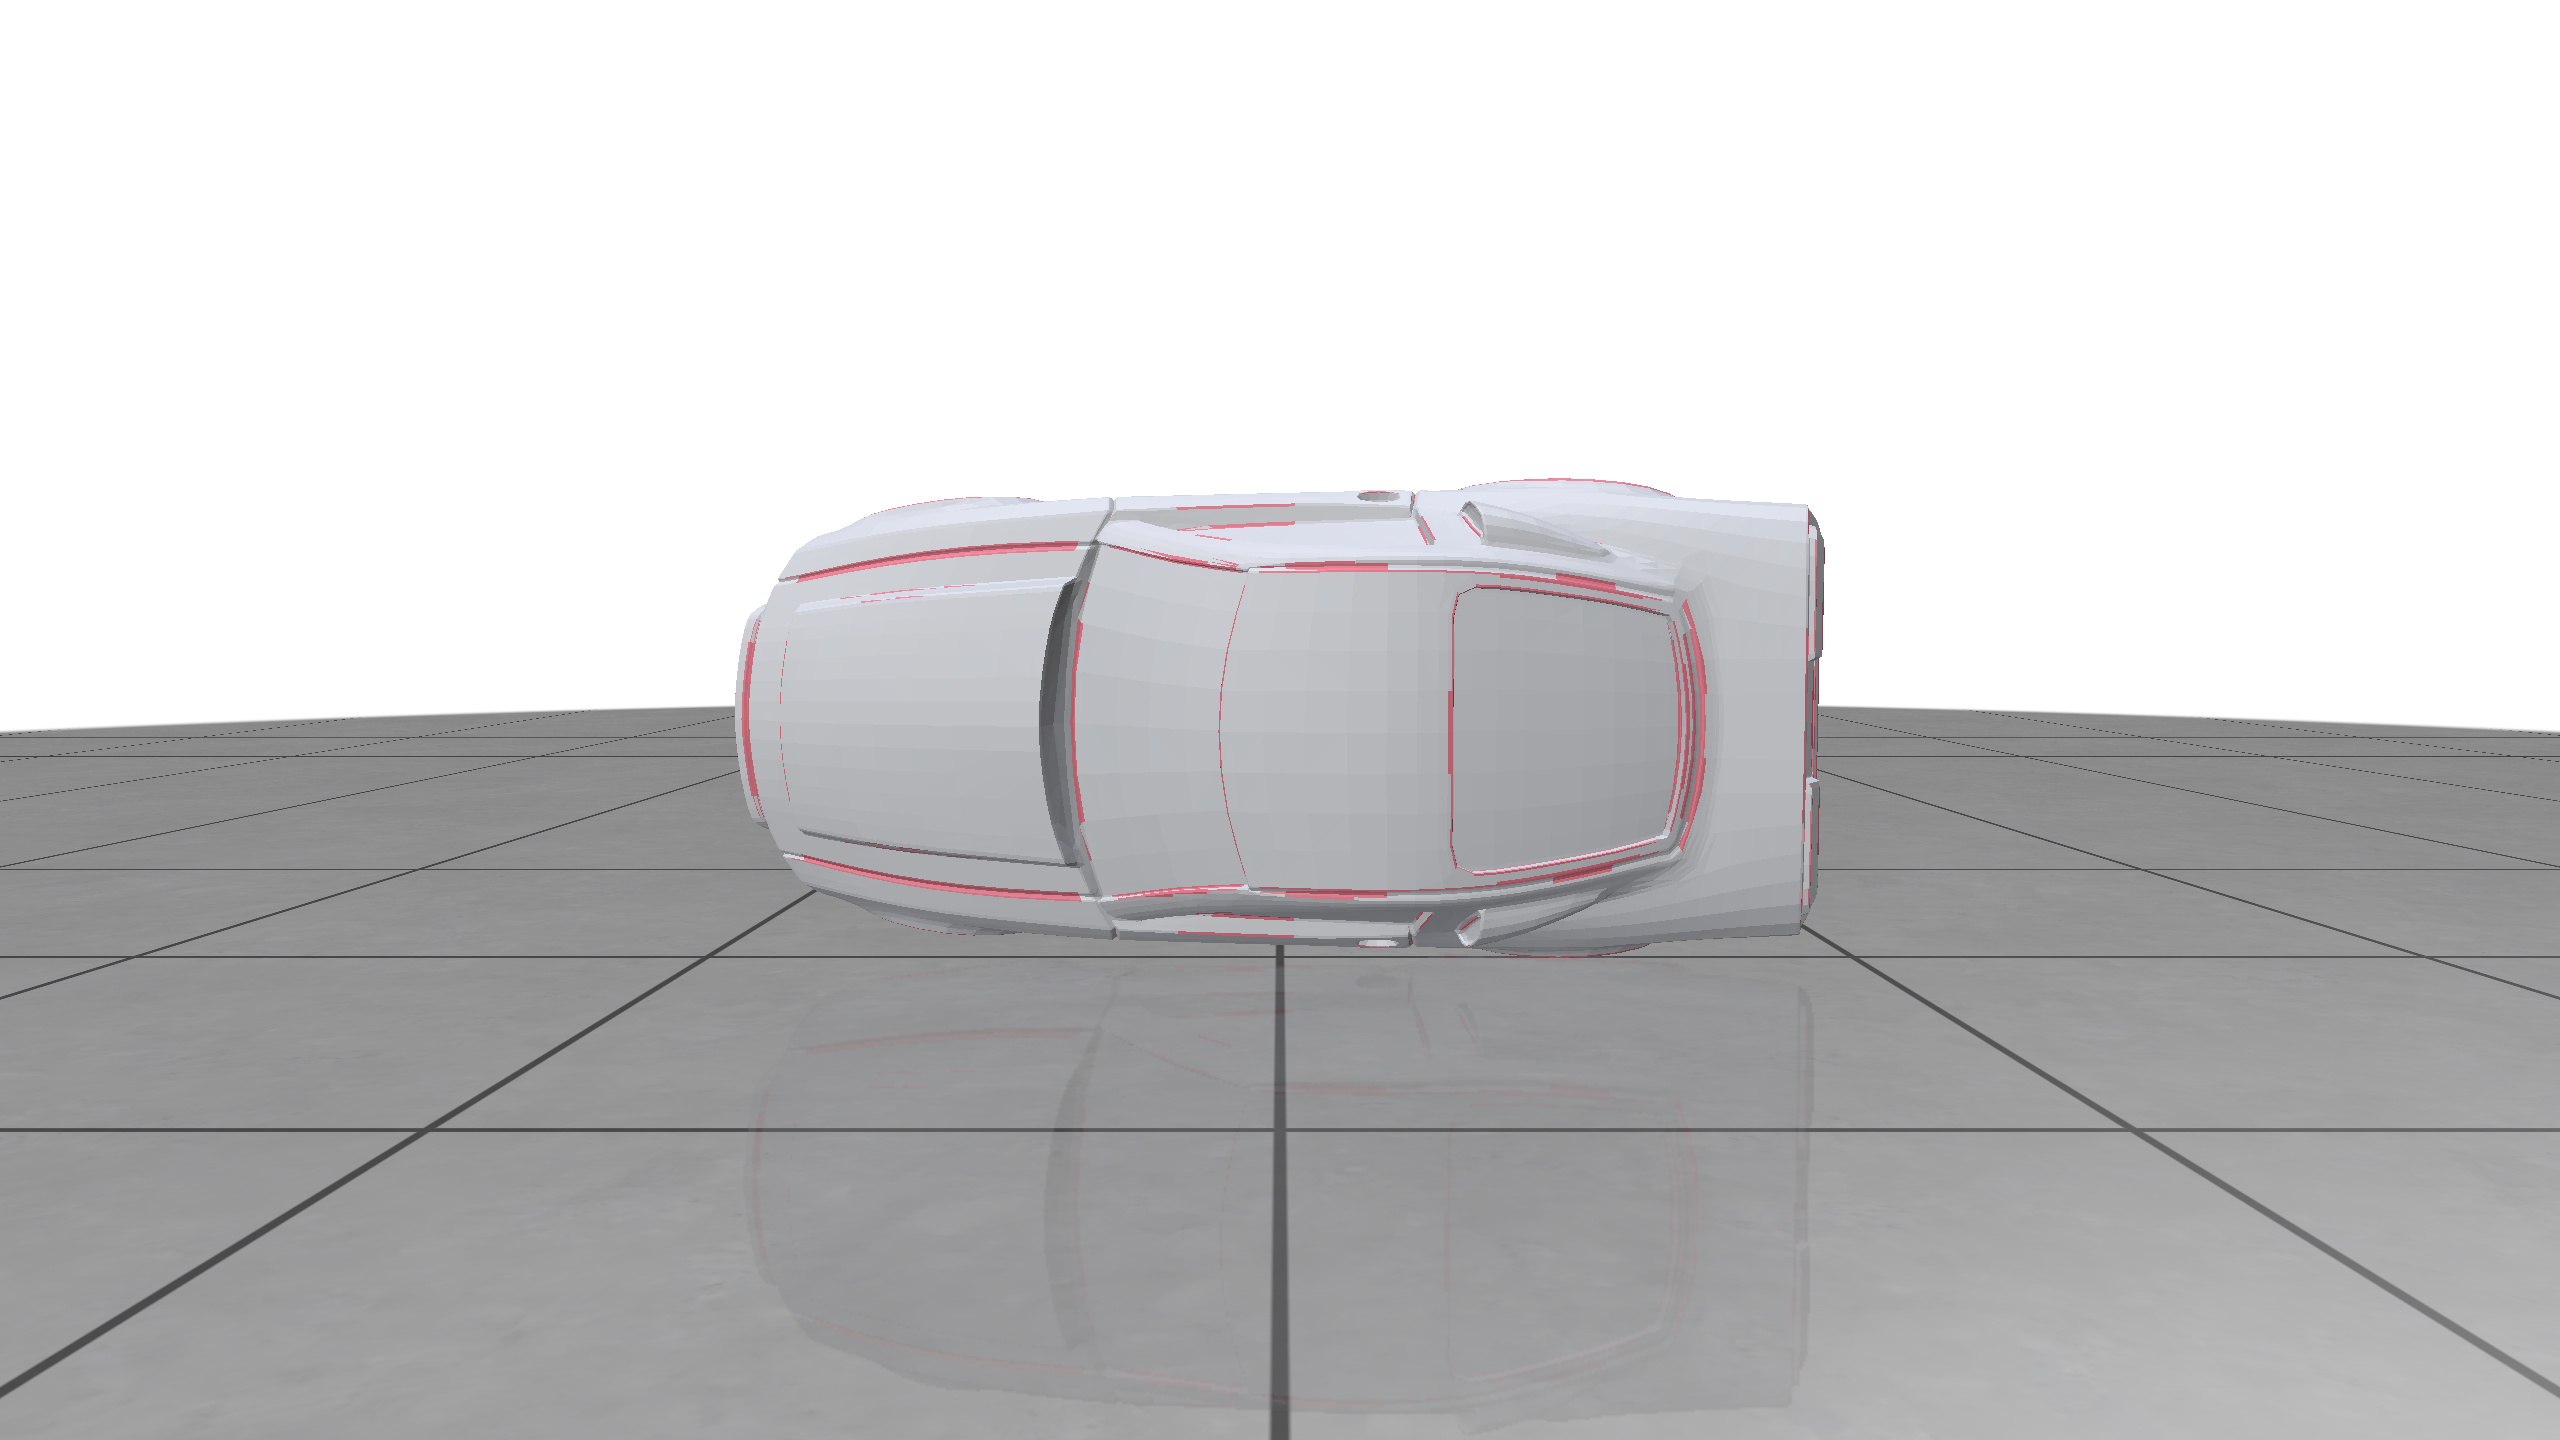
\includegraphics[width=\linewidth]{fig05_car4_input_quality.png}
    \caption{\code{car4.off}}
  \end{subfigure}
  \hfill
  \begin{subfigure}{0.48\linewidth}
    \centering
    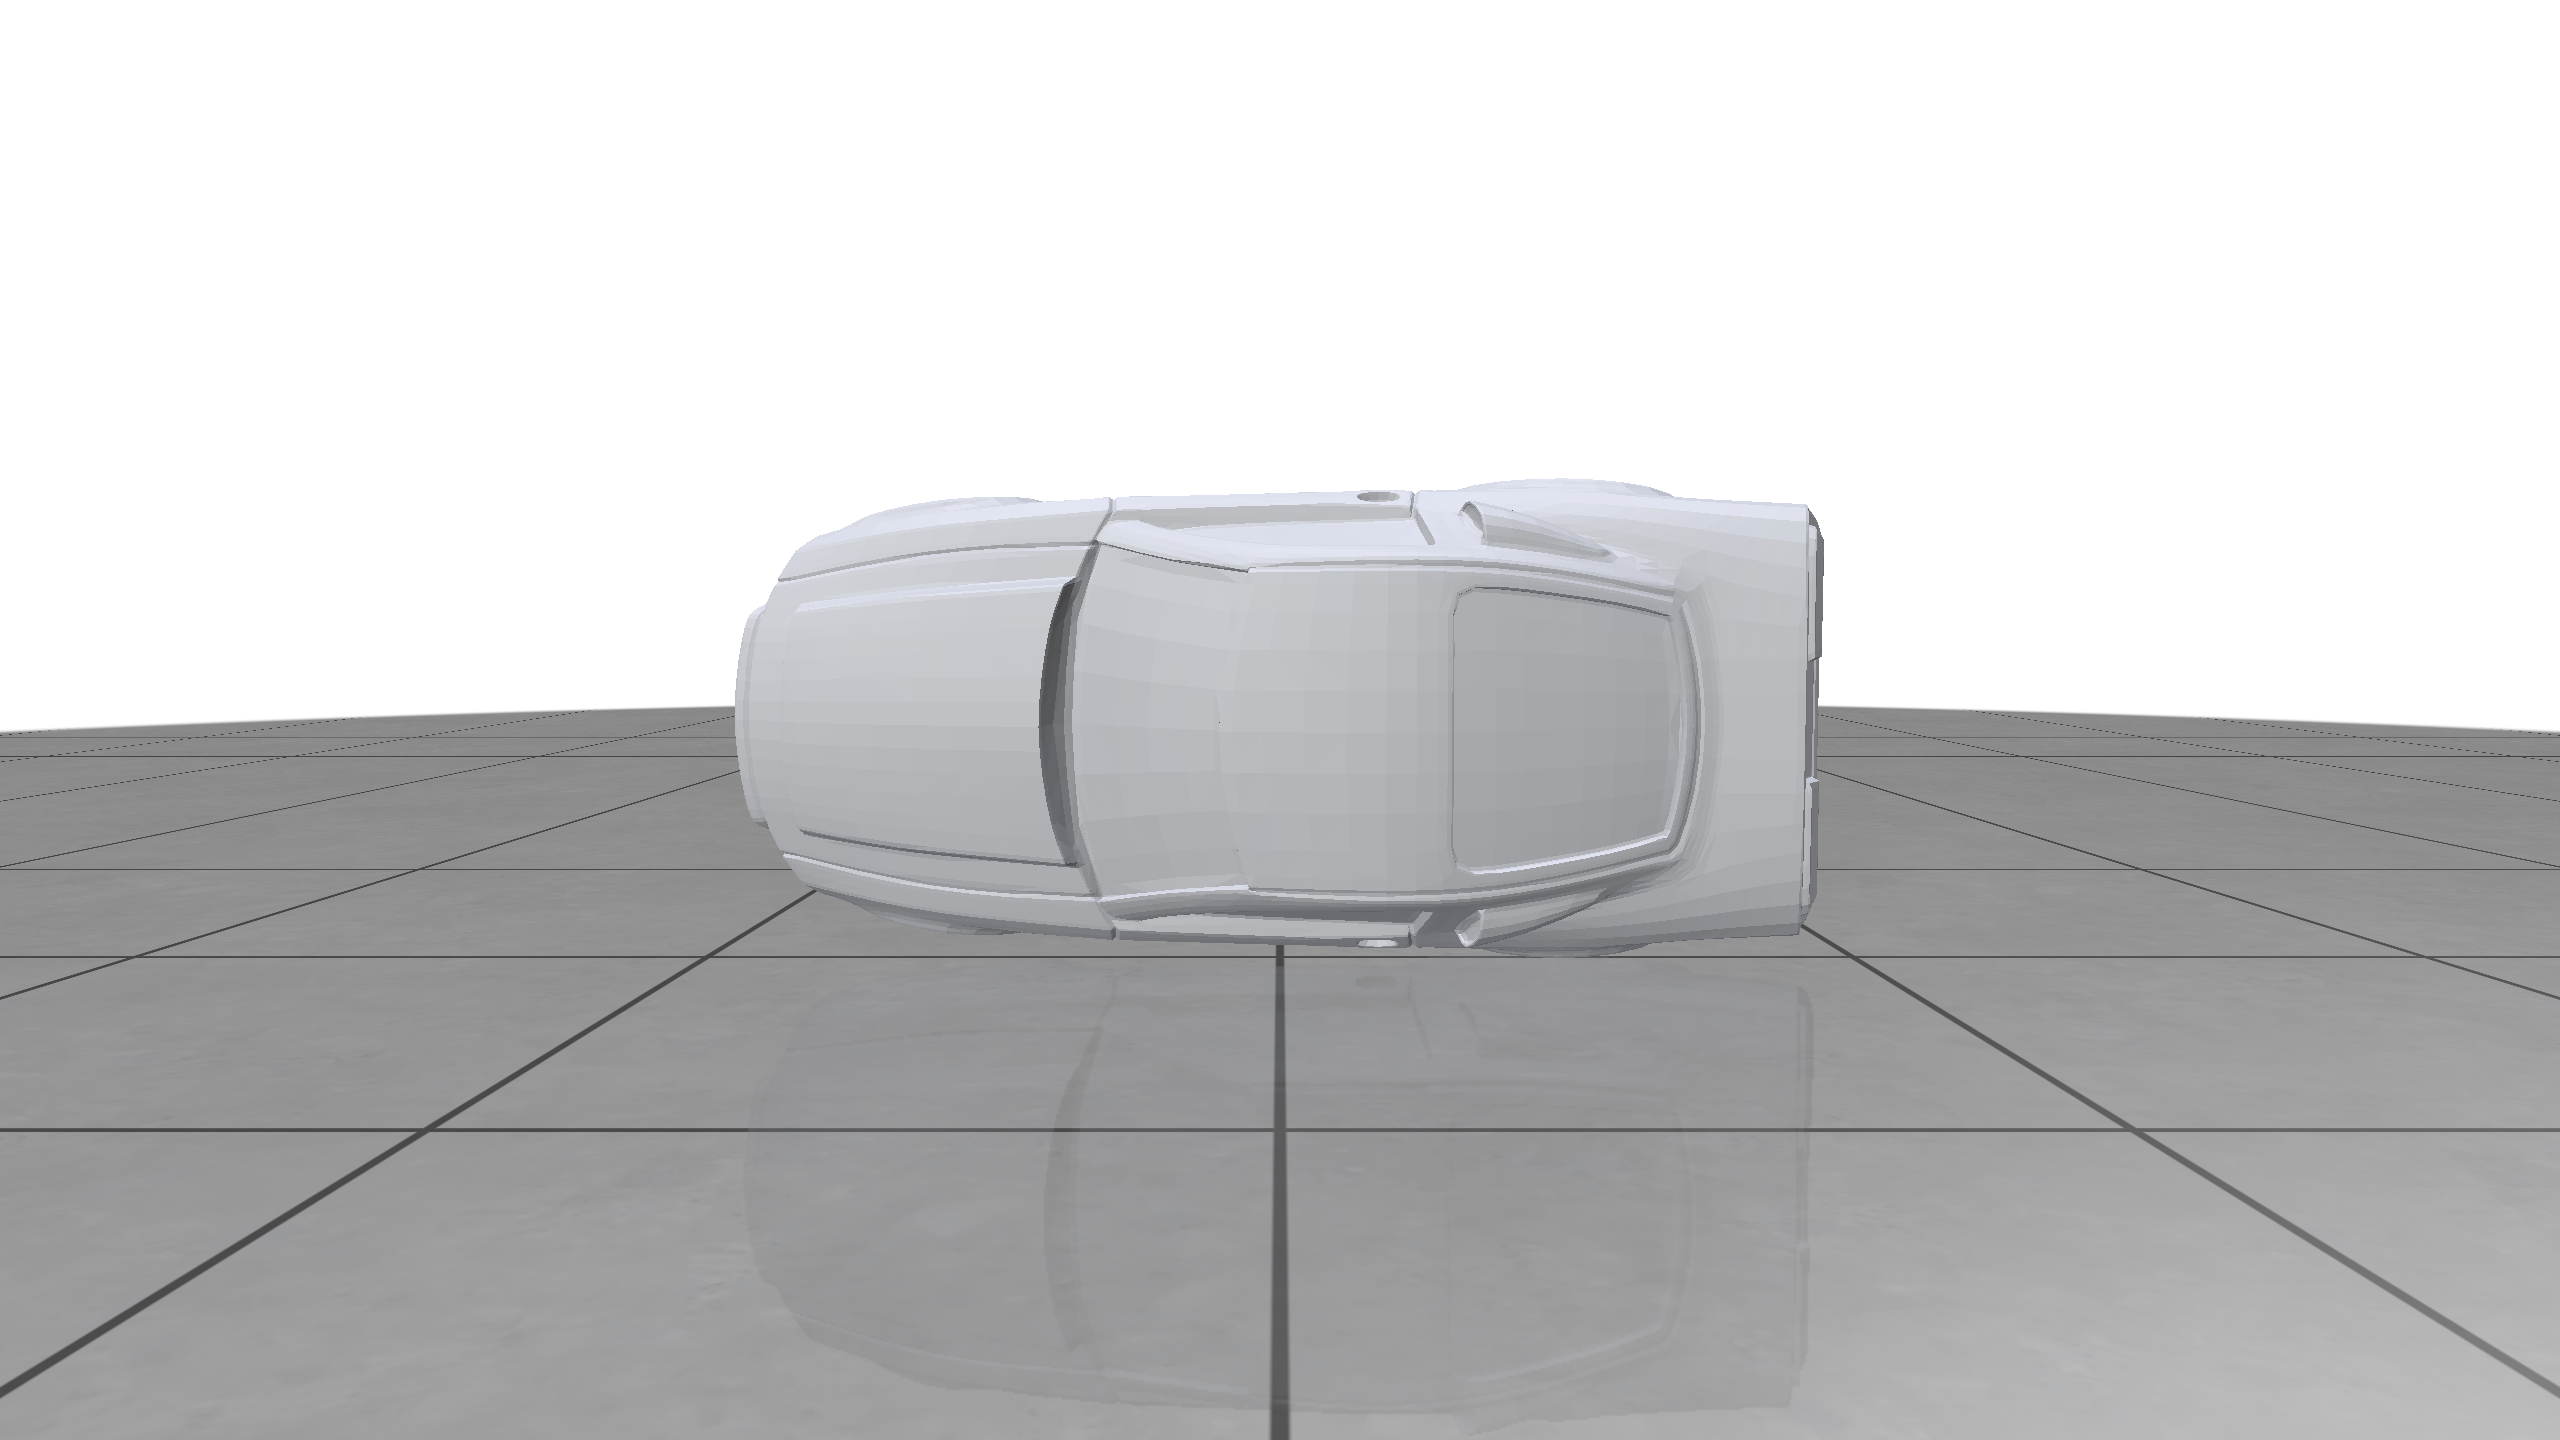
\includegraphics[width=\linewidth]{fig06_car4_cleanup_quality.png}
    \caption{\code{car4\_cleanup.off}}
  \end{subfigure}
  \caption{Car4 before and after targeted cleanup. The bad triangle count is reduced from 4787 to 5.}
  \label{fig:car4}
\end{figure}

\begin{figure}[H]
  \centering
  \begin{subfigure}{0.48\linewidth}
    \centering
    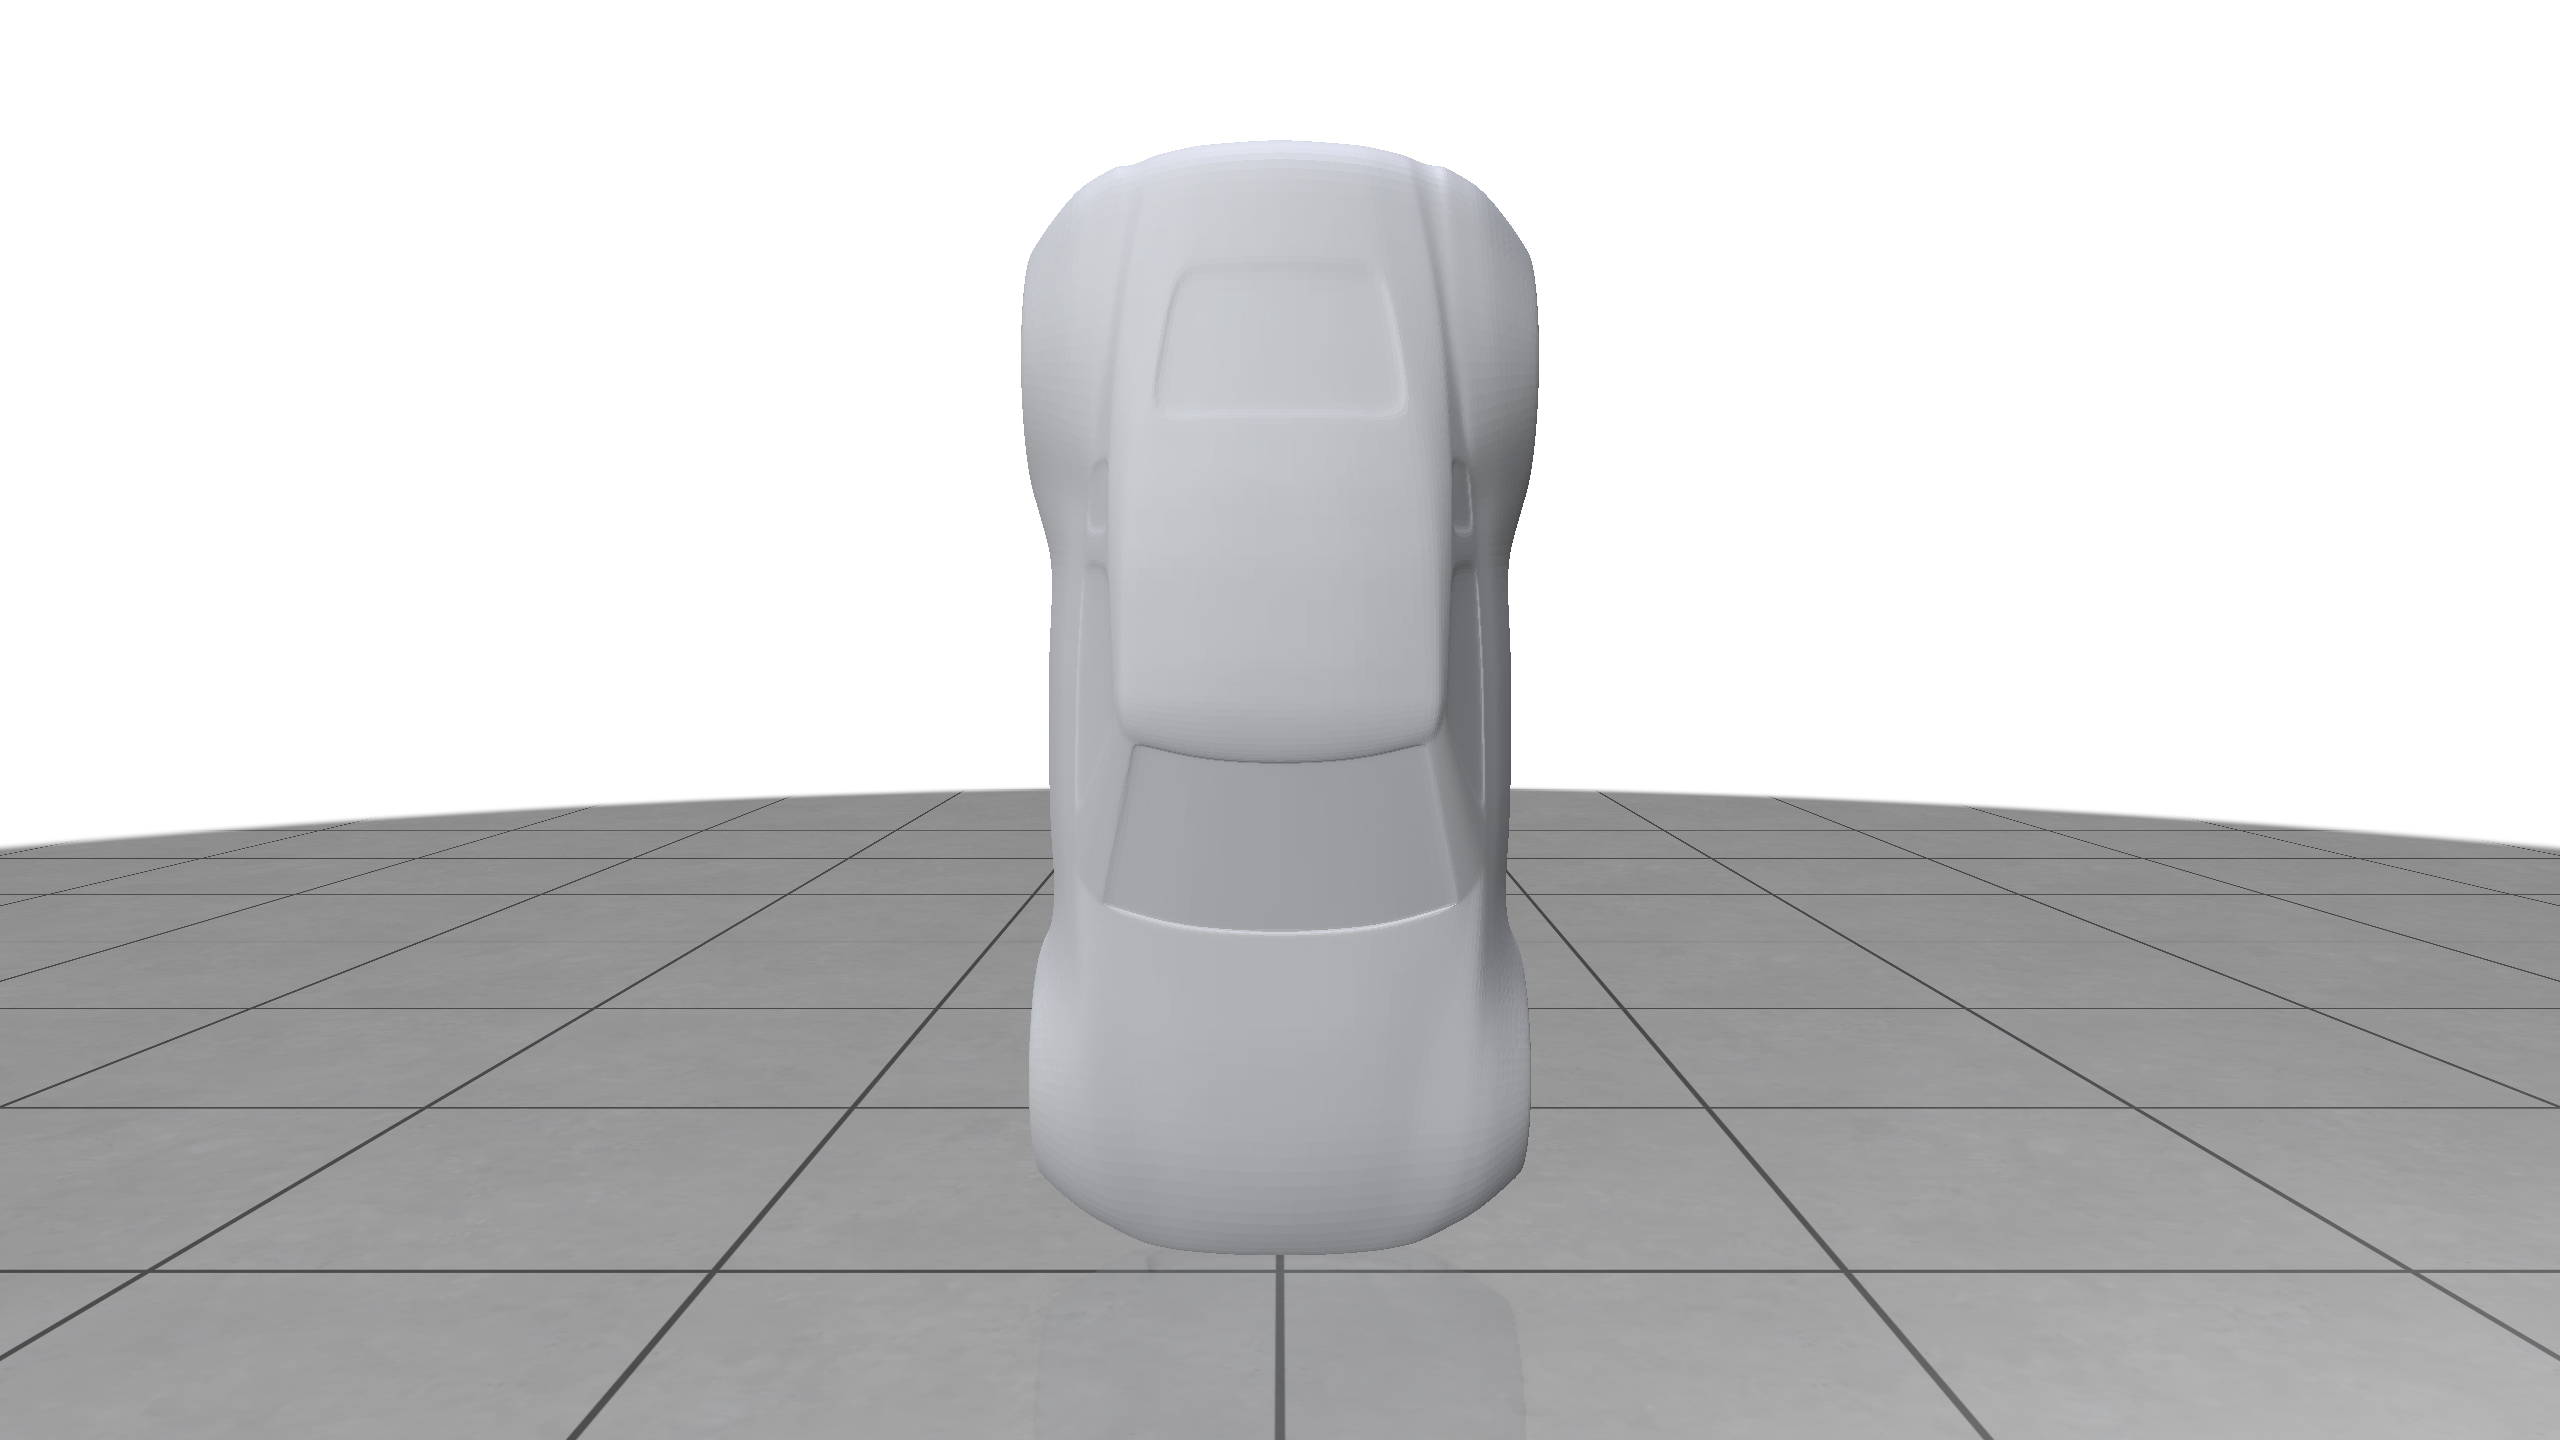
\includegraphics[width=\linewidth]{fig07_car1_input_quality.png}
    \caption{\code{car1.off}}
  \end{subfigure}
  \hfill
  \begin{subfigure}{0.48\linewidth}
    \centering
    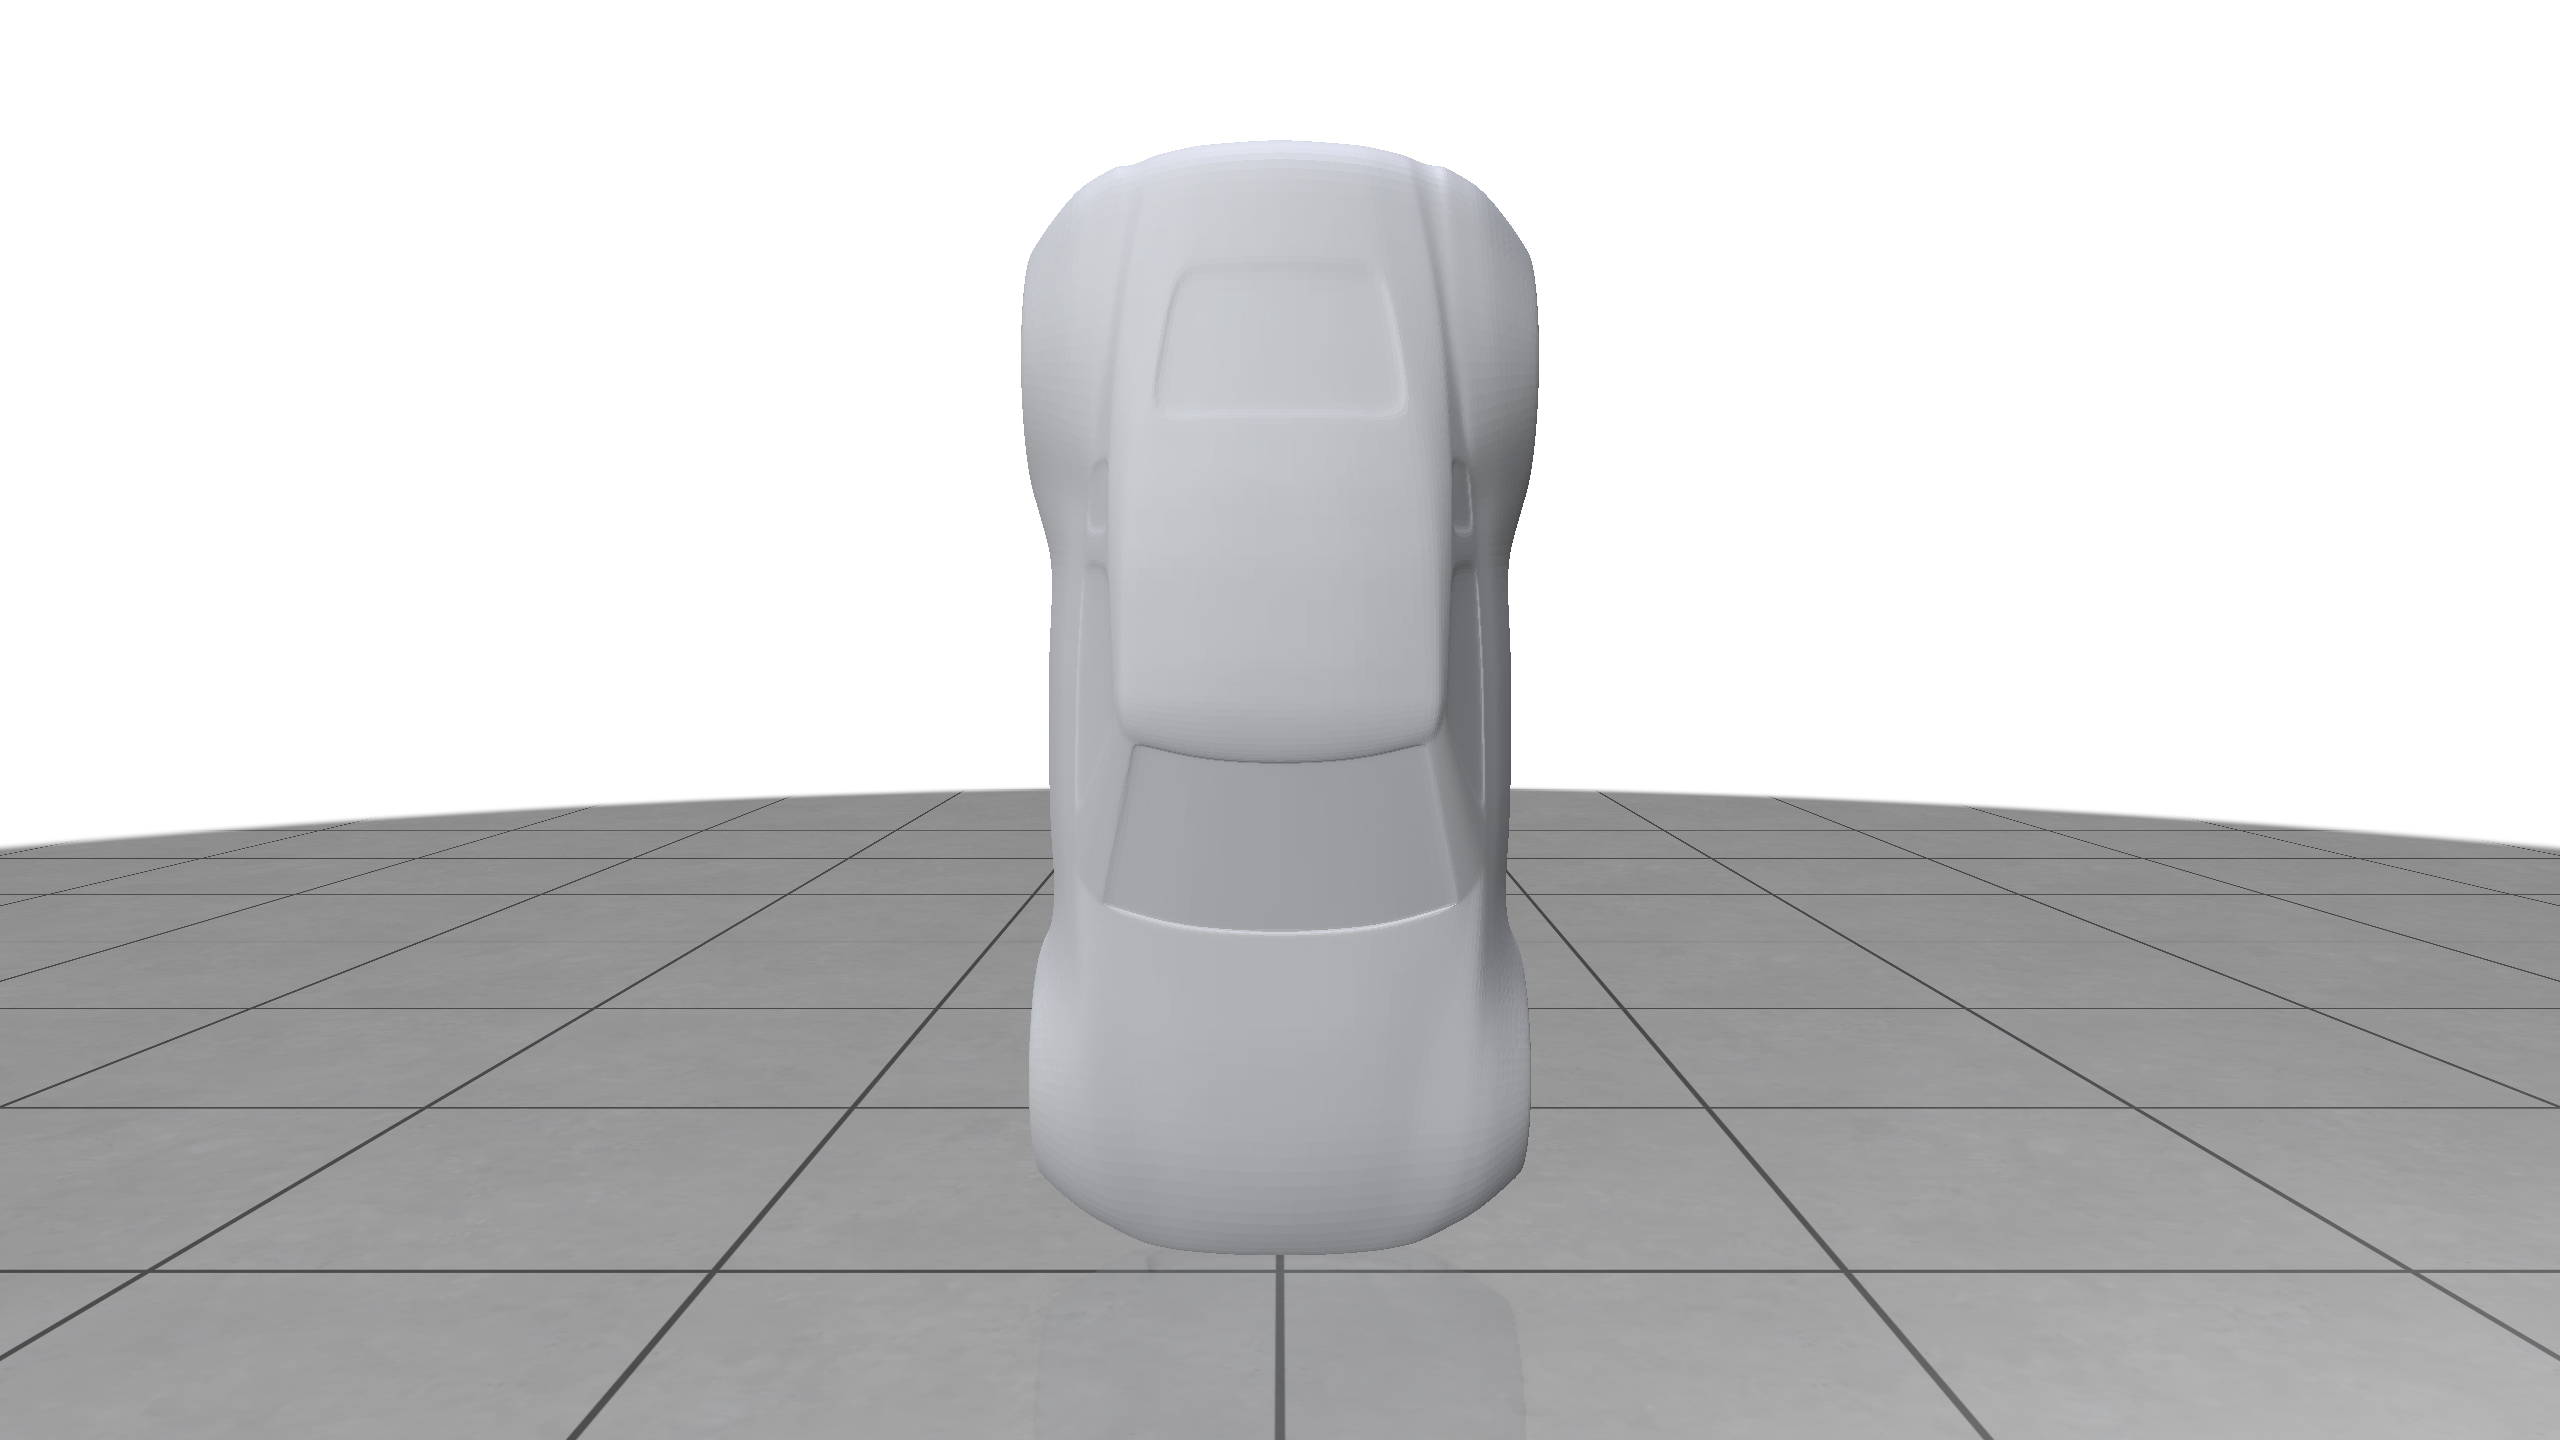
\includegraphics[width=\linewidth]{fig08_car1_cleanup_quality.png}
    \caption{\code{car1\_cleanup.off}}
  \end{subfigure}
  \caption{Car1 before and after targeted cleanup. The input already has boundary edges, and the cleanup preserves the boundary count.}
  \label{fig:car1}
\end{figure}

\section{Encountered Problems and Observations}

Several implementation issues were useful for understanding the problem:

\begin{enumerate}
  \item \textbf{Naive splitting can break topology.} The first remeshing attempt split individual triangles independently. This created missing faces and visible cracks. The fix was globally consistent edge splitting.

  \item \textbf{Improving triangle angles is not enough.} Some early outputs had better angle statistics but worse topology. This is why boundary and non-manifold edge counts are reported in all experiments.

  \item \textbf{Smoothing may deform the shape.} Laplacian-like smoothing improved triangle regularity but visibly changed the object. Projection back to the original surface helped, but the final conservative pipeline avoids relying on smoothing.

  \item \textbf{Cleanup should be type-specific.} Splitting the longest edge of every bad triangle made some cases worse. The better rule was to collapse shortest edges for needles and split longest edges for caps.

  \item \textbf{Adaptive remeshing is useful but sensitive.} It improved the joint result, but on larger car models it over-refined the mesh without additional acceleration or better parameter control.

  \item \textbf{Feature preservation remains important.} Some small bumps near sharp edges remain visible. This is expected because explicit feature-edge preservation using dihedral angles is not implemented.
\end{enumerate}

\section{Limitations}

This project deliberately keeps the method simple and transparent. The main limitations are:
\begin{itemize}
  \item no explicit feature-edge preservation,
  \item no exact Hausdorff-distance error bound,
  \item no spatial acceleration for nearest-surface or adaptive operations,
  \item cleanup stopping criteria are still parameter-based,
  \item adaptive remeshing parameters are tuned manually.
\end{itemize}

These limitations are acceptable for the scope of the term project, but they also suggest clear future improvements.

\section{Conclusion}

The project produced a working and measurable mesh-quality enhancement pipeline. The implemented method successfully removes all detected bad triangles from the provided joint input mesh while preserving topology. It also performs well on additional car models, reducing thousands of detected bad triangles to only a few remaining cases without introducing non-manifold edges.

The most important lesson from the project is that robust mesh processing should not be evaluated only by visual appearance or triangle-angle statistics. Topology preservation, failure cases, and parameter sensitivity must also be measured. The final pipeline reflects this lesson: it combines quality analysis, visualization, conservative operations, targeted cleanup, and adaptive remeshing into a reproducible workflow.

\section{Reproducibility}

The main commands are documented in \code{README.md}. The code is organized under the \code{meshfix/} package and can be run from the project root using:

\begin{verbatim}
python3 -m meshfix.cli
\end{verbatim}

Important output files include:
\begin{itemize}
  \item \code{outputs/meshes/joint\_adaptive\_final.off}
  \item \code{outputs/meshes/car1\_cleanup.off}
  \item \code{outputs/meshes/car4\_cleanup.off}
  \item \code{outputs/experiment\_summary.csv}
  \item \code{outputs/joint\_adaptive\_final\_metrics.csv}
\end{itemize}

\bibliographystyle{plain}
\bibliography{references}

\end{document}
